\documentclass[english,xcolor=svgnames]{beamer}

\input{../../../../Templates/Latex/teachingslidesbeamer.tex}



%%%%%%%%%%%%%%%%%%%%%%%%%%%%%%%%%%%%%%%%%%%%%%%%%%
\AtBeginSection[]{
\setbeamertemplate{footline}{}
  \frame<beamer>{ 

    \frametitle{Outline}   

    \tableofcontents[currentsection] 
  }
\setbeamertemplate{footline}[frame number]{}
\addtocounter{framenumber}{-1}
}

\AtBeginSubsection[]{
\setbeamertemplate{footline}{}
  \frame<beamer>{ 

    \frametitle{Outline}   

    \tableofcontents[currentsection,currentsubsection] 
  }
  \setbeamertemplate{footline}[frame number]{}
  \addtocounter{framenumber}{-1}
}

% ===========================================================
% ===========================================================
% ===========================================================
\begin{document}

\title{One Period Nominal Rigidity}
\vspace{1cm}
\author[shortname]{
\begin{tabular}{c}
	Johannes Wieland \\ 
	\footnotesize \href{mailto:jfwieland@ucsd.edu}{jfwieland@ucsd.edu}  \\ 
\end{tabular}
}

\date{Spring \the\year}

\setbeamertemplate{footline}{}
\makebeamertitle
\setbeamertemplate{footline}[frame number]{}

\addtocounter{framenumber}{-1}

\section{Introduction}

\begin{frame}
\frametitle{Introduction
}
\begin{itemize}
	\item The data consistently showed real effects of monetary policy on output, at least in the short-run.
	\item Our previous model was inconsistent with this data.
	\item We will now modify our a model so that prices are fixed for one period.
	\begin{itemize}
		\item Important is that prices do not adjust in response to new information (e.g., increase in money supply).
		\item The ``simple'' model provides intuition for more complex models of nominal rigidity that we will see later in class.
%		\begin{itemize}
%			\item Insights very similar to those of the standard new Keynesian model.
%		\end{itemize}
	\end{itemize}
%	\item For now we will drop money in the utility function.
\end{itemize}
\end{frame}

\section{Sticky Prices}

\begin{frame}
\frametitle{Sticky Prices
}
\begin{itemize}
	\item We assume that prices are fixed at time $1$ (today):
	\begin{align*}
		P_1 = P_0 \\
	\end{align*}
	where $P_0$ is the past price level.
	\begin{itemize}
		\item Implicit assumption: Firm will supply whatever output is demanded at the price the firm set.
		\item May not be a good assumption in certain circumstances. Why would a firm want to operate at a loss?
		\item Fixed cost models are more compelling in this regard. We may study these later in the course, time-permitting.
	\end{itemize}
\end{itemize}	
\end{frame}



\begin{frame}
\frametitle{How does the Labor Market Clear?
}
\begin{itemize}
	\item At time $t=1$ firms, must hire however many workers they need to fulfill demand $\Rightarrow$ Households on labor supply curve.
	\begin{align*}
		\frac{W_1}{P_0}&=\frac{\chi N_1^\varphi}{C_1^{-\gamma}}
	\end{align*}
	\item But firms are not on their labor demand curve:
	\begin{align*}
		\frac{W_1}{P_0}&\neq   A_1  = MPL_1
	\end{align*}
	\item Firms will hire as many workers as needed to produce the output demand at price $P_0$.
\end{itemize}	
\end{frame}

\begin{frame}
\frametitle{Why Sticky Prices?
}
\begin{center}
	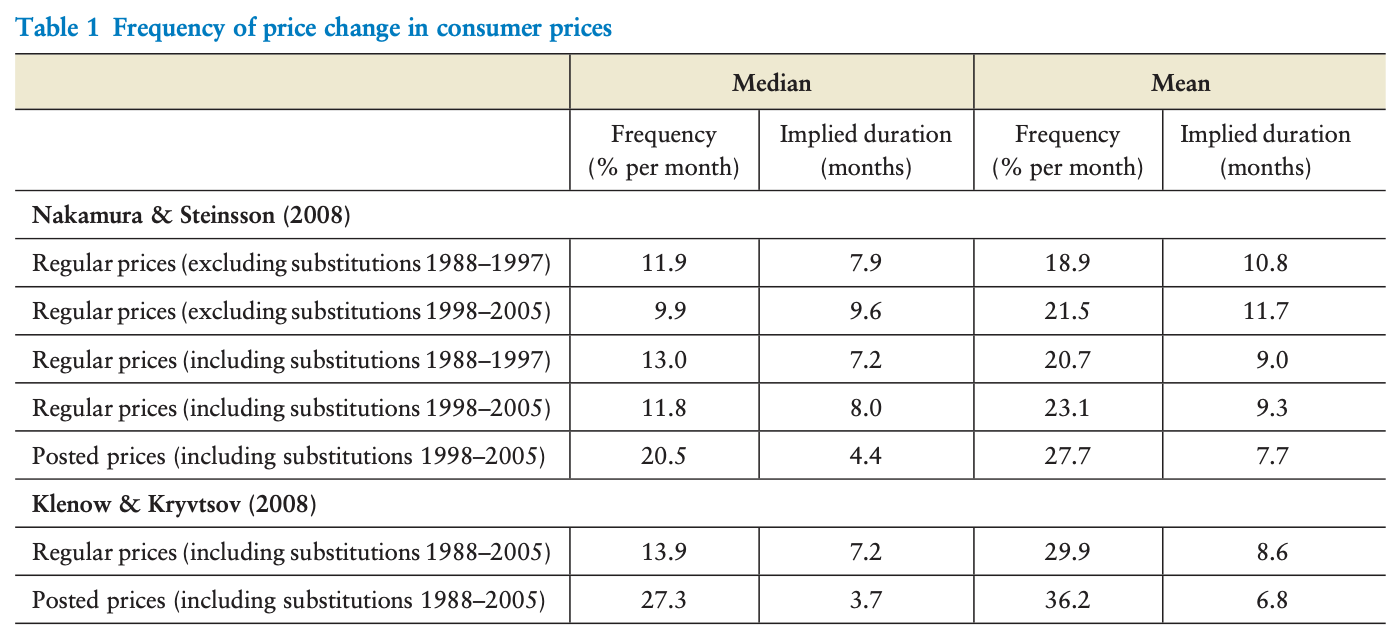
\includegraphics[scale=0.5]{../../images/NS2013frequency.png}
\end{center}
\begin{itemize}
	\item Source: Nakamura and Steinsson (2013)
\end{itemize}	
\end{frame}

\begin{frame}
\frametitle{Other Approaches
}
\begin{itemize}
	\item Similar (but not identical) results obtain if we assume sticky wages. See your homework.
	\item We will study more sophisticated sticky price approaches later in class.
	\begin{itemize}
		\item Insights will often be quite similar.
	\end{itemize}
	\item Time-permitting, we will also cover the sticky information approach to monetary (non-)neutrality.
	\item What is key in all these approaches is that some price / value is indexed to money (the unit of account).
\end{itemize}	
\end{frame}


\begin{frame}
\frametitle{Equilibrium Equations: Long-run}
\begin{itemize}
	\item Long-run $=$ $t\ge 2$:
\end{itemize}
\begin{align*}
	Y_t&=A_tN_{t}  \\
	\frac{W_t}{P_t}&= A_t  \\
	\frac{W_t}{P_t}&=\frac{\chi N_t^\varphi}{C_t^{-\gamma}} \\
	Y_t&=C_t \\
	\frac{M_t}{P_t}&=\zeta^{1/\nu}\left(1-\frac{1}{Q_t}\right)^{-1/\nu}C_{t}^{\gamma/\nu}\\
	1&=\beta E_t\left\{Q_t \frac{P_t}{P_{t+1}} \frac{C_{t+1}^{-\gamma}}{C_{t}^{-\gamma}}\right\} 
\end{align*}
\begin{itemize}
	\item Classical Dichotomy holds in the long-run.
\end{itemize}
\end{frame}


\begin{frame}
\frametitle{Equilibrium Equations: Short-run}
\begin{itemize}
	\item Short-run (period 1):
\end{itemize}
\begin{align*}
	Y_1&=A_1N_{1}  \\
	\color{red}P_1&\color{red}= P_0  \\
	\frac{W_1}{P_1}&=\frac{\chi N_1^\varphi}{C_1^{-\gamma}} \\
	Y_1&=C_1 \\
	\frac{M_1}{P_1}&=\zeta^{1/\nu}\left(1-\frac{1}{Q_1}\right)^{-1/\nu}C_{1}^{\gamma/\nu}\\
	1&=\beta E_1\left\{Q_1 \frac{P_1}{P_{2}} \frac{C_{2}^{-\gamma}}{C_{1}^{-\gamma}}\right\} 
\end{align*}
\begin{itemize}
	\item Sticky price assumption replaces labor demand curve.
\end{itemize}
\end{frame}




\begin{frame}
\frametitle{Simplifying assumptions
}
\begin{itemize}
	\item All exogenous variables constant for $t\ge 2$:  $A_t=A$, $M_t=M$. 
	\item There is perfect foresight for these paths.
	\item[$\Rightarrow$] Solve for steady state values for $C_2=C$ and $P_2=P$ and plug into short-run solution.
	\item At $t=1$ we then ``shock'' $M_1$ and $A_1$ and see what happens to $C_1,Y_1,P_1$.
\end{itemize}	
\end{frame}


\begin{frame}
\frametitle{Solution: Long-run}
\begin{itemize}
	\item Solve for the steady state:
\end{itemize}
\begin{align*}
	C = Y &=\left[\frac{1}{\chi} A^{1 + \varphi}\right]^{\frac{1}{\gamma + \varphi}} \\
	\frac{M}{P}&=\zeta^{1/\nu}\left(1-\beta\right)^{-1/\nu}Y^{\gamma/\nu}
\end{align*}
\begin{itemize}
	\item Classical Dichotomy holds in the long-run.
	\begin{itemize}
		\item Any change in $M$ causes a proportional change in $P$, leaving $Y,C$ unchanged.
	\end{itemize}
\end{itemize}
\end{frame}


\begin{frame}
\frametitle{Equilibrium Equations: Short-run}
\begin{itemize}
	\item Short-run (period 1):
\end{itemize}
\begin{align*}
	Y_1&=A_1N_{1}  \\
	\frac{W_1}{\color{red} P_0}&=\chi N_1^\varphi Y_1^{\gamma} \\
	\frac{M_1}{\color{red} P_0}&=\zeta^{1/\nu}\left(1-\frac{1}{Q_1}\right)^{-1/\nu}Y_{1}^{\gamma/\nu}\\
	1&=\beta \left\{Q_1 \frac{\color{red} P_0}{\color{red} P} \frac{\color{red} Y^{-\gamma}\color{black}}{Y_{1}^{-\gamma}}\right\} 
\end{align*}
%\begin{itemize}
%	\item From Euler equation, changes in the \emph{nominal} interest rate $Q_1$ have a direct effect on output and consumption $Y_1 = C_1$.
%	\item For given level of $Y_1$ can manipulate \emph{nominal} interest rate by changing the money supply $M_1$
%	\item[$\Rightarrow$] Classical Dichotomy does not hold in short-run. 
%\end{itemize}
\end{frame}

\begin{frame}
\frametitle{Equilibrium Equations: Short-run}
\begin{itemize}
	\item Short-run (period 1):
\end{itemize}
\begin{align*}
	C_1 = Y_1&= \left\{ \frac{1}{\beta Q_1} \frac{\color{red} P}{\color{red} P_0} \right\}^{\frac{1}{\gamma}} Y \\
	\frac{M_1}{\color{red} P_0}&=\zeta^{1/\nu}\left(1-\frac{1}{Q_1}\right)^{-1/\nu}Y_{1}^{\gamma/\nu}\\
\end{align*}
\begin{itemize}
	\item From Euler equation, changes in the \emph{nominal} interest rate $Q_1$ have a direct effect on output and consumption $Y_1 = C_1$.
	\item For given level of $Y_1$ can manipulate \emph{nominal} interest rate by changing the money supply $M_1$
	\item[$\Rightarrow$] Classical Dichotomy does not hold in short-run. 
\end{itemize}
\end{frame}



\begin{frame}
\frametitle{Intuition
}
\begin{enumerate}[1.]
	\item Higher $M_t$ reduces real rate $R_{t+1}=Q_t (P_t/P_{t+1})$:
	\begin{itemize}
		\item Nominal rate $Q_t$ falls to induce households to hold the extra money supplied.
		\item Expected inflation is fixed because current prices $P_t$ are sticky, and future prices $P_{t+1}$ are determined by future $M$.
	\end{itemize}
	\item Lower real rate increases demand today through intertemporal substitution:
	\begin{enumerate}[(a)]
		\item Low return on savings, so increase today's consumption relative to future consumption.
		\item But future consumption is fixed by the supply-side as prices are flexible.
		\item So there is an overall increase in consumption today, which is accommodated by firms hiring more workers and producing more output.
	\end{enumerate}
\end{enumerate}
\end{frame}


\begin{frame}
	\frametitle{Intution (2)
	}
	\begin{itemize}
		\item Households do \emph{not} spend the extra money. They hold it.
		\begin{itemize}
			\item In our model households get utility from holding money.
		\end{itemize}
		\item Household budget constraint shows how it adds up:
		\begin{align*}
			C_t + \frac{B_{t}}{P_t}  + \frac{M_t}{P_t}  \le \frac{W_t}{P_t} N_t +  \frac{Q_{t-1}B_{t-1}}{P_t} + \frac{M_{t-1}}{P_t} + TR_t+PR_t
		\end{align*}
		\begin{itemize}
			\item Households carry more money $\frac{M_t}{P_t}$.
			\item This is financed by additional government transfers $TR_t$.
			\item When the government prints money it gives it to the households through transfers.
		\end{itemize}
		\item From household money demand we know that households are only willing to hold the extra money (rather than spend it), if the nominal interest rate falls.
	\end{itemize}
\end{frame}

\begin{frame}
	\frametitle{Intution (3)
	}
	\begin{itemize}
		\item The mechanism is intertemporal substitution: a lower real interest rate means the household wants to consume more today and save less. 
		\item But the household does not end up consuming less in the future ($C_2=Y$). 
		\item In fact in equilibrium savings do not change and are equal to zero.
		\item This has to be the case: in our model there is no way for households to transfer output from one period to the next.
		\item What happens is that household income in period 1 rises because firms produce more output to meet the demand.
		\item This allows the household to consume more today without needing to reduce their (zero) saving.
	\end{itemize}
\end{frame}
	

\begin{frame}
\frametitle{Equilibrium Equations: Short-run}
\begin{itemize}
	\item Short-run (period 1):
\end{itemize}
\begin{align*}
	C_1 = Y_1&= \left\{ \frac{1}{\beta Q_1} \frac{\color{red} P}{\color{red} P_0} \right\}^{\frac{1}{\gamma}} Y \\
	\frac{M_1}{\color{red} P_0}&=\zeta^{1/\nu}\left(1-\frac{1}{Q_1}\right)^{-1/\nu}Y_{1}^{\gamma/\nu}\\
	Y_1&=A_1N_{1}  
\end{align*}
\begin{itemize}
	\item From Euler equation, the level of output $Y_1 = C_1$ is pinned down by $Q_1$.
	\item Changes in productivity $A_1$ have no effect on real output.
%	\item[$\Rightarrow$] Output is ``demand-determined.''
	\item Higher productivity $A_1$ reduces employment $L_1$.
\end{itemize}
\end{frame}

\begin{frame}
\frametitle{Intuition
}
\begin{enumerate}[3.]
	\item Why does productivity not affect output? Because it does not affect the real interest rate and therefore does not affect consumption demand.
	\item Employment falls because demand is fixed and with higher productivity we do not need as much labor to produce the same output.
\end{enumerate}
\end{frame}


\begin{frame}
\frametitle{Summary
}
\begin{itemize}
	\item With sticky prices, classical dichotomy no longer holds in the short-run.
	\begin{itemize}
		\item But it does hold in the long-un.
	\end{itemize}
	\item The jargon in the literature is:
	\begin{itemize}
	\item In the short-run output is ``demand-determined'': nominal interest rates and the nominal money supply determine output, but not productivity or labor-supply preferences.
	\item In the long-run output is ``supply-determined'': only productivity, technology, and preferences determine output.
	\end{itemize}
\end{itemize}

\end{frame}


\section{Evidence}


\begin{frame}
\frametitle{Basu et al. (2006): ``Purifying'' The Solow Residual}
\begin{itemize}
	\item Difficult to measure $A_t$: lots of unobserved variation in input intensity of labor capital.
%	\item Newer, more econometrically sophisticated measure of technology controlling for capital and labor utilization.
	\item Basu, Fernald, and Kimball (2006):
	\begin{itemize}
		\item Control for aggregation effects, varying utilization of $K$ and $L$, non-constant returns to scale, imperfect competition.
		\item Varies half as much as Solow Residual.
		\item Shocks are permanent and serially uncorrelated.
	\end{itemize}
	\item What happens when technology improves?
\end{itemize}
\end{frame}


\begin{frame}
\frametitle{Basu et al. (2006): Solow Residual}
\centering
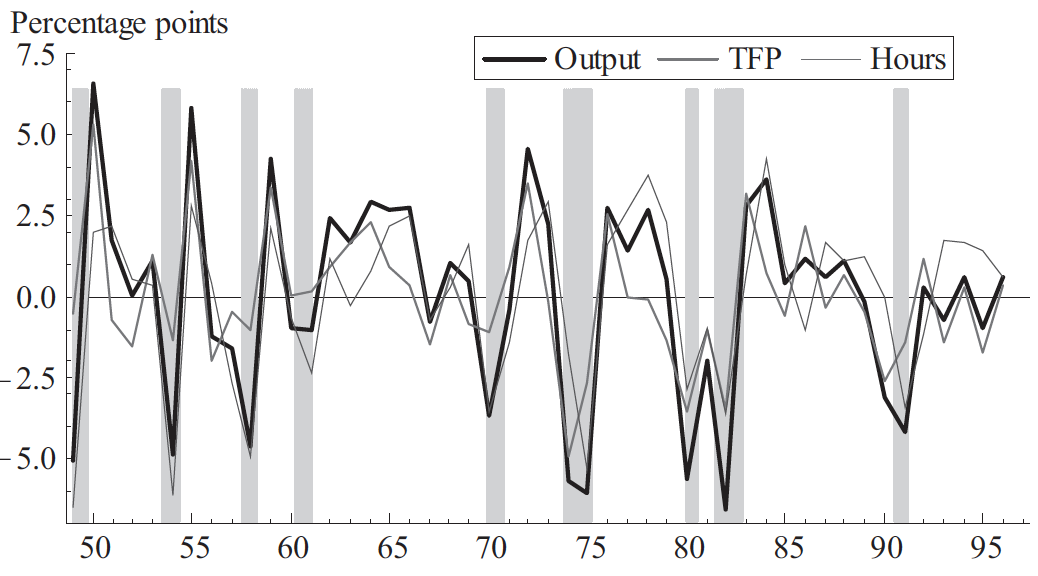
\includegraphics[scale=0.6]{../../Images/BFK2006TFP.png}	
\end{frame}

\begin{frame}
\frametitle{Basu et al. (2006): Technology}
\centering
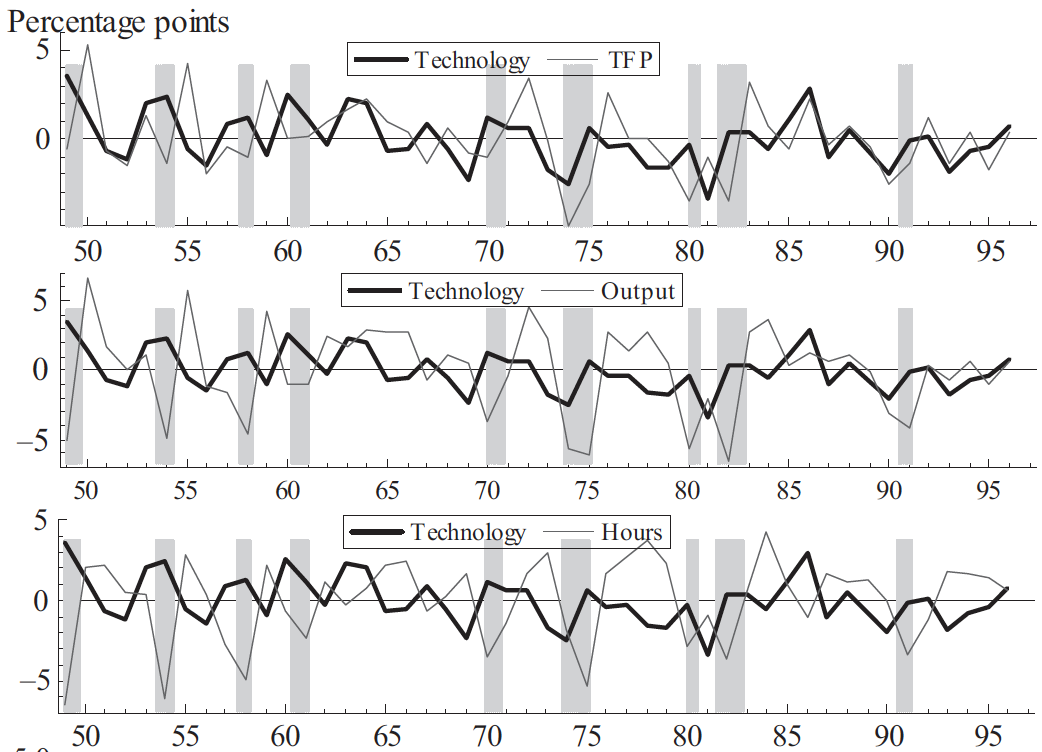
\includegraphics[scale=0.6]{../../Images/BFK2006Technology.png}	
\end{frame}

 
\begin{frame}
\frametitle{Labor Market and Labor Wedge
}
\begin{itemize}
	\item The distortion (implicit tax) in the labor market is called the \emph{labor wedge:}
	\begin{align*}
		(1-\tau_t^N)\equiv\frac{MRS_t}{MPL_t}=\frac{\chi N_t^\varphi C_t^{\gamma}}{(1-\alpha)Y_t/N_t}
	\end{align*}
	\item $\tau_t^N=0$ (no distortion) when:
	\begin{itemize}
		\item Firms are on their labor demand equation.
		\item Households are on their labor supply equation.
		\item Perfect competition.
	\end{itemize}
%	Before we closed the model by combining labor supply and labor demand,
%	\begin{align*}
%		\frac{\chi N_t^\varphi}{C_t^{-\gamma}}&=\frac{(1-\alpha)A_t N_t^{-\alpha}}{(1+\mu_t)}
%	\end{align*}
%		\item But now firms no longer on labor demand curve.
%		\item The endogenous mark-up (labor wedge) makes this equation always hold. (Like an identity rather than an equilibrium relationship.)
%		\item This is good: in the data the labor wedge moves endogenously with the business cycle.
\end{itemize}

\end{frame}


\begin{frame}
\frametitle{Finding: $\tau_t^N$ is Countercyclical}
	\begin{align*}
		\tau_t^N = 1- \frac{MRS_t}{MPL_t} \Rightarrow MPL_t>MRS_t \text{ in Recessions }
	\end{align*}
	\centering
	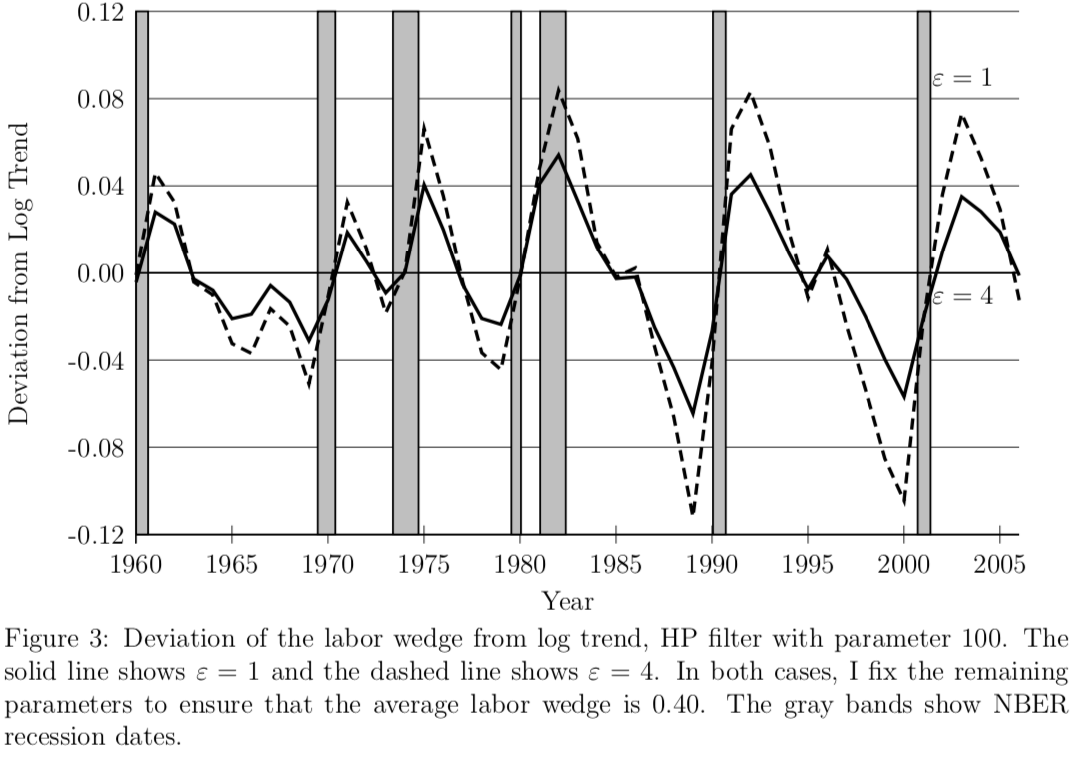
\includegraphics[scale=0.5]{../../Images/Shimer2009laborwedge.png}
\end{frame}

\begin{frame}
\frametitle{Labor Wedge In Our Sticky Price Model}
\begin{itemize}
	\item The labor wedge at $t=1$ is:
	\begin{align*}
		(1-\tau_1^N)\equiv\frac{MRS_t}{MPL_t}=\chi A_1^{\gamma-1}   N_1^{\gamma + \varphi} 
	\end{align*}
	\item In a recession $N_1$ is low and labor wedge is high. This is consistent with the data.
%	\begin{itemize}
%		\item Argument assumes recessions are not caused by productivity changes.	
%	\end{itemize}
	\item Important: labor market distortion does not have to originate in the labor market. Here the problem is a sticky price in the output market.
\end{itemize}
\end{frame}



\section{Next Steps}

\begin{frame}
\frametitle{Next Steps
}
\begin{itemize}
	\item Who sets prices? Why are they rigid?
	\item Develop New Keynesian model that relaxes several assumptions we have made.
	\item For next class, read Gali Ch. 3. 
\end{itemize}
\end{frame}


\end{document}